\section{Results}\label{sec:results}
For our experiments, we used a Red Hat 8 server with a Intel Xeon Gold 6242
CPU. Since \shortname{} is written in Rust, it mostly uses the built-in
functionality of the egg library. The egg e-graph runner was ran in a
time-limited configuration, meaning there was no limit in the size of the
e-graph or number of rewrite iterations. The specific time limit for e-graph
construction was 10 minutes. In most cases, the test circuit saturated the
e-graph well before this time limit---around 30 seconds. \shortname{} was
evaluated against circuits from three benchmark suites: EPFL~\cite{epflbench},
ISCAS'85~\cite{iscasbench}, and LGSynth'91~\cite{lgsynthbench}. However, we
also included an ALU and pipelined multiplication module to test how our
compiler behaves with increasing levels of bit-parallelism and pipeline stages.
Finally, we measure how our mapping optimizations influence CLB usage and
timing closure.

\subsection{Benchmarking}\label{sec:results:benchmark}
\begin{table}
    \centering
    \csvautobooktabular{data/results.csv}
    \caption{Results of \nimproved{} improved benchmarks from ISCAS'85~\cite{iscasbench}, LGSynth'91~\cite{lgsynthbench}, and EPFL~\cite{epflbench}}\label{tab:results}
\end{table}

\begin{figure}
    \begin{subfigure}{0.47\textwidth}
        \centering
        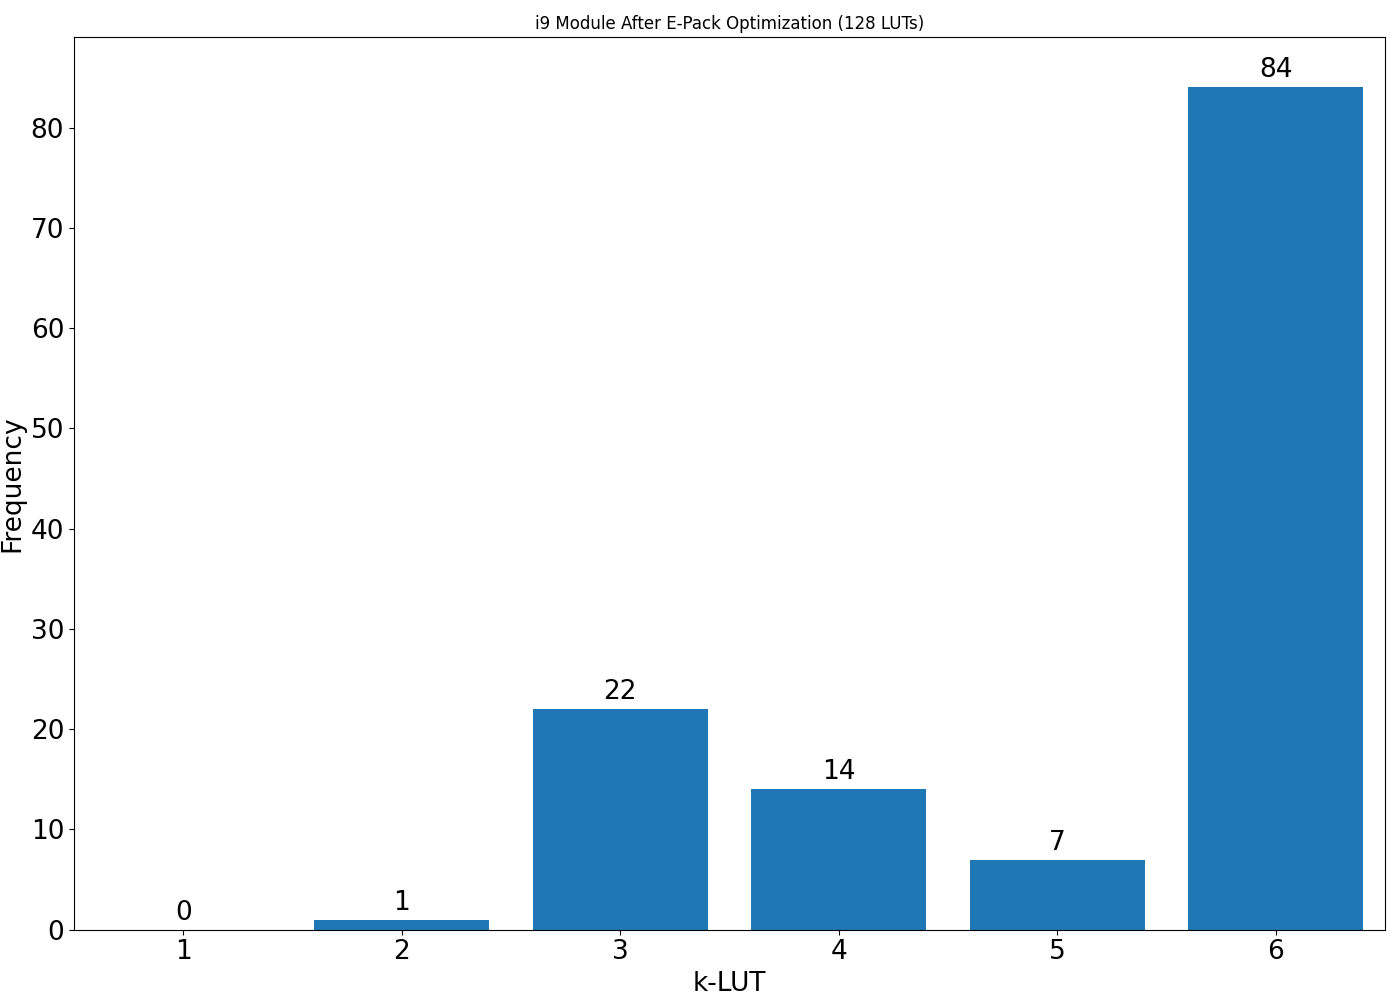
\includegraphics[width=\textwidth]{img/y33.png}
        \caption{Distribution of 150 LUTs after synthesis of `i9' with Yosys 0.33}\label{fig:histogram:y33}
    \end{subfigure}
    \hfill\vspace{4mm}
    \begin{subfigure}{0.47\textwidth}
        \centering
        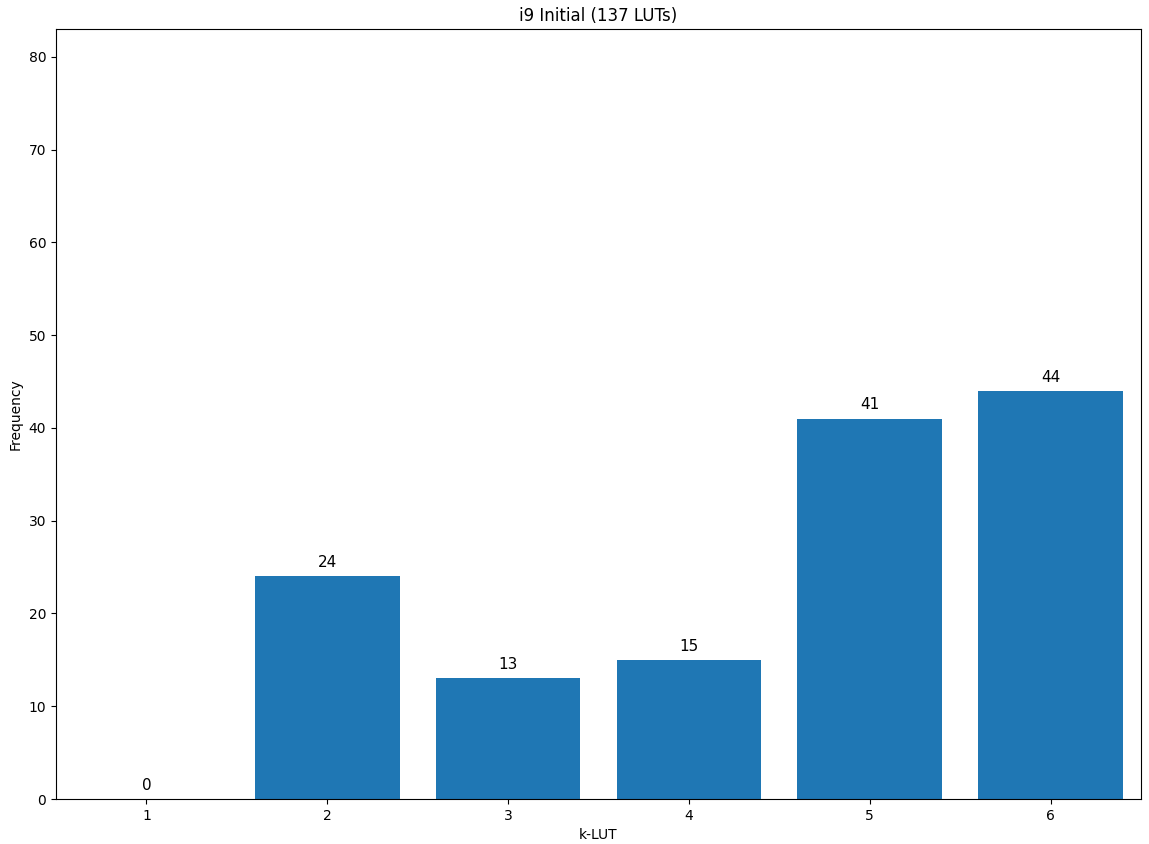
\includegraphics[width=\textwidth]{img/y44.png}
        \caption{Distribution of 137 LUTs after synthesis of `i9' with Yosys 0.44}\label{fig:histogram:y44}
    \end{subfigure}
    \hfill\vspace{4mm}
    \begin{subfigure}{0.47\textwidth}
        \centering
        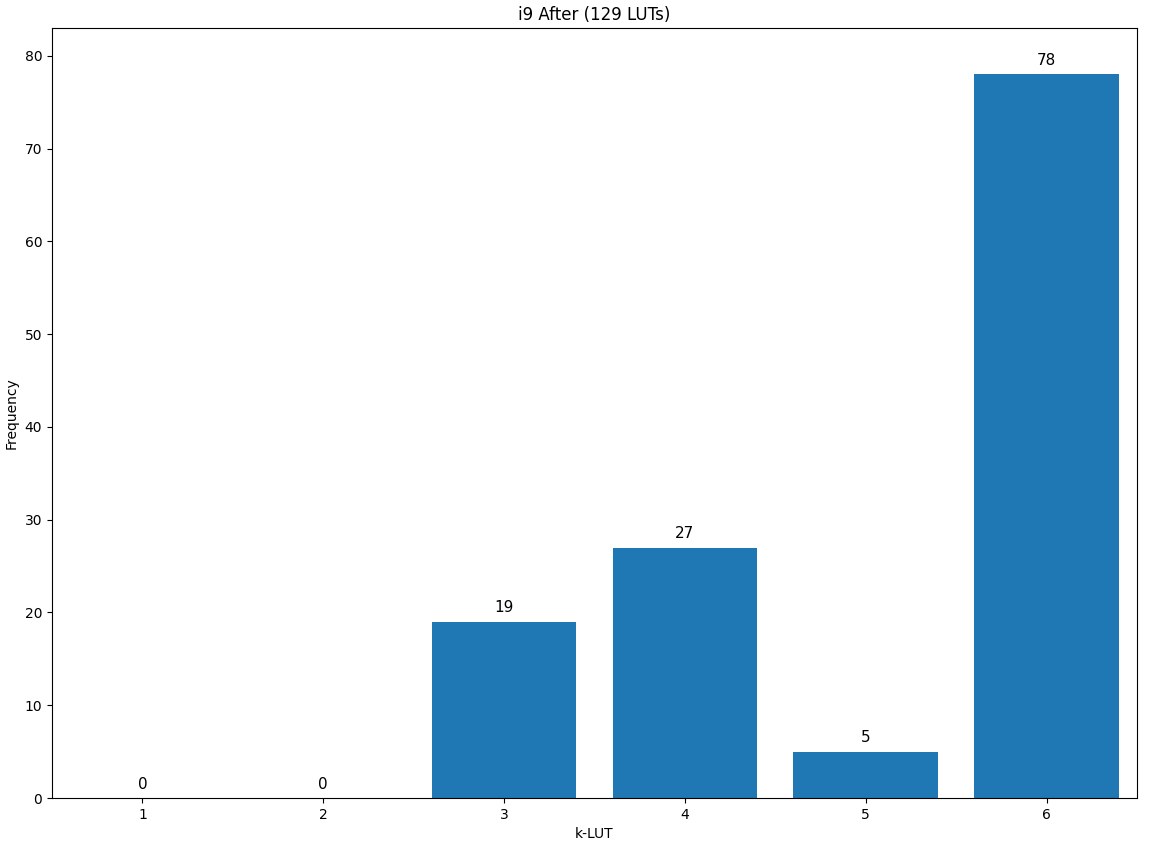
\includegraphics[width=\textwidth]{img/epack.png}
        \caption{Distribution of 129 LUTs after synthesis of `i9' with Yosys 0.3 + \shortname{}}\label{fig:histogram:epack}
    \end{subfigure}
    \caption{Comparison of two initial structures, (a) and (b), and E-Packed structure (c) \todo{regenerate these figs}}\label{fig:histogram}
\end{figure}

We used an compilation of \nbenchmarks{} combinational benchmarks from three
academic sources to test LUT packing ability. Among the combinational
benchmarks we tested, \shortname{} was able to reduce the LUT count \fmetric{}
of the time. On average, \shortname{} packed the netlists to \metric{}. The
results in Table~\ref{tab:results} list all the reduced LUT counts, sorted by
approximate design size. AMD/Xilinx Vivado 2022~\cite{vivado} was used as the
baseline synthesis tool. For the E-Pack flow, Yosys~\cite{yosys} is used to
generate the initial mapped circuit. At a glance, circuits like `int2float,'
`c6288,` `adder,' and `square' have the most to gain from \shortname{}. These
circuits are all arithmetic in nature, and this is a recurring point of
emphasis throughout the rest of the results.

One result that is \textit{not} demonstrated by the table is the apparent
importance of the initial structure inputted to E-Pack. We have not eliminated
all sources of structural bias, and hence our superoptimization tool still
occasionally gets stuck at a local minimum. Fig.~\ref{fig:histogram}
illustrates the issue by depicting the different distributions of $k$-LUT usage
by different tool flows. In short, an overly packed LUT network will fare worse
in attempts to superoptimize it. Future work will investigate which qualities
make an RTL synthesis engine work well with our tool versus ones that do not.
For example, E-Pack optimized Yosys 0.33 netlists
(Fig.~\ref{fig:histogram:y33}) better than ones provided by Yosys 0.47
(Fig.~\ref{fig:histogram:y44}). A future version of \shortname{} should
implement new rewrite procedures than can break out of these local minimums on
their own.

\subsection{Marginal Improvement and Cost}\label{sec:results:margin}
\begin{figure}
    \begin{subfigure}{0.47\textwidth}
        \centering
        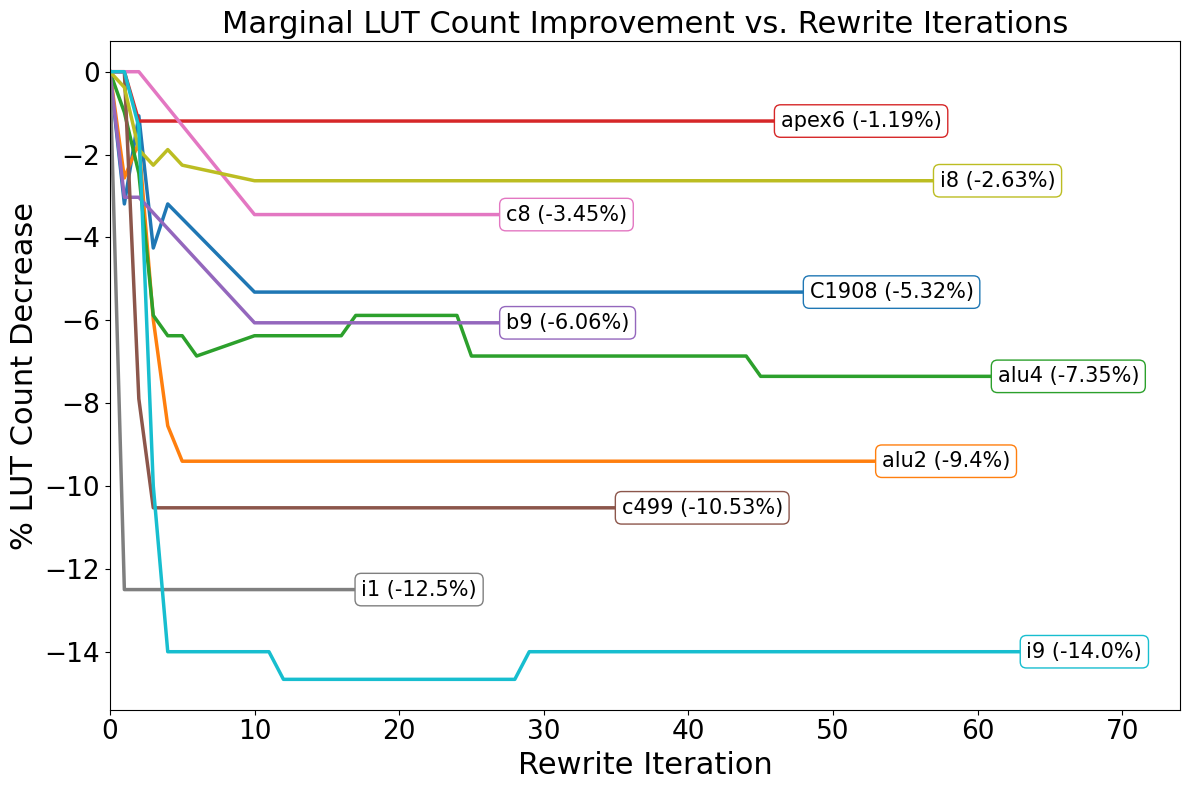
\includegraphics[width=\textwidth]{img/improvement.png}
        \caption{Marginal improvement versus iteration count. The labels mark the equality saturation point.}\label{fig:marginal:improvement}
    \end{subfigure}
    \hfill\vspace{4mm}
    \begin{subfigure}{0.47\textwidth}
        \centering
        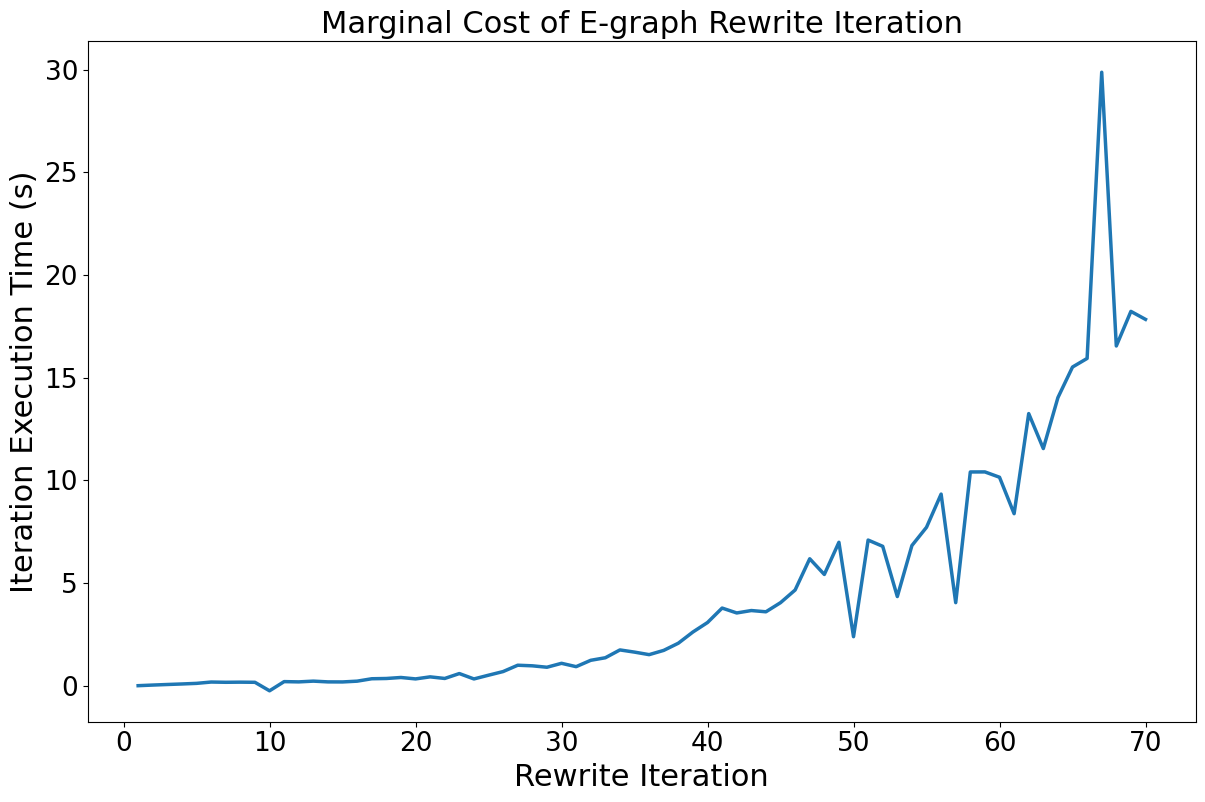
\includegraphics[width=\textwidth]{img/runtime_derivative.png}
        \caption{Marginal increase in runtime versus iteration count. Later iterations consume more time as the graph is larger.}\label{fig:marginal:runtime}
    \end{subfigure}
    \caption{Comparison of gains in QoR against e-graph size and runtime. Running a netlist to equality saturation requires more rewrite iterations, and hence a larger e-graph.}\label{fig:marginal}
\end{figure}

Given that \shortname{} is fundamentally a superoptimization tool, we want to
provide evidence that significant gains can be found within reasonable time
bounds. To that end, we empirically studied the marginal gains in QoR as the
e-graph contains increasingly longer rewrite sequences. Within the e-graph
infrastructure, this phasing of applying rewrites and rebuilding the union-find
data structure is known as an \textit{iteration}. As shown in
Fig.~\ref{fig:marginal:improvement}, nearly all the performance gains are
discovered within the first 10 iterations---well before equality
saturation---suggesting that most of the optimizations are relatively local.
Some notable exception occur, such as `alu4' being reduced in size after the
40th iteration. Lastly, the growing runtime of e-graph exploration with each
iteration should be addressed. The marginal cost of executing an iteration of
rewrites becomes prohibitive as the e-graph becomes larger.
Fig.~\ref{fig:marginal:runtime} illustrates that after approximately the 30th
iteration, the marginal runtime rapidly increases into the 10s of seconds.

\subsection{Case Study: Pipelined Designs}\label{sec:results:retiming}
\begin{table*}[t]
    \centering
    \csvautobooktabular{data/mult.csv}
    \caption{LUT and flip-flop counts are report post-synthesis, but before placement and routing. CLB counts are reported after placement and routing.}\label{tab:multiply}
\end{table*}

Hardware designs with feed forward pipelines provide interesting opportunities
to apply register retiming and find a higher-level of area optimization. When
closing timing on FPGA designs, the critical path is often dominated by the
effects of routing congestion, moreso than ASIC design. Hence, reducing the
cell count and circuit depth along the delay path is a valid optimization
strategy for FPGA design. As a caveat, it is important to note that other work
has also observed the opposite trend~\cite{academicfpga}: decreasing depth too
much can strain the router. In any case, E-Pack can be utilized to reduce total
CLB usage. To elaborate, every CLB in the Ultrascale+ architecture contains 1
slice, which itself contains 8 LUTs and 16 flip-flops~\cite{ug574}.
Intuitively, a design that maps to CLBs efficiently will contain more
flip-flops than LUTs due to this 2:1 ratio. To test this hypothesis,
Table~\ref{tab:multiply} shows the results of a 32-bit pipelined multiplier
with a varying number of pipeline stages processed with E-Pack.

While the total drop is CLB usage is desirable, the area gains as a percentage
are modest due to the suboptimality of greedy e-graph extraction. Register
retiming rewrites, when enabled, vastly increase the design space. More
importantly, register retiming changes the topology of the stateful
elements---i.e. the flip-flops. As a consequence, greedy extraction cannot take
into account the fanout of flip-flops. It chooses a poor design point with less
register fanout and a greater total number of registers. The few regressions
observed in mapping combinational logic (Fig.~\ref{fig:marginal:improvement})
become more frequent and exacerbated in sequential logic. While these results
\textit{do} demonstrate that optimizing for CLB count over raw cell count is a
feasible strategy, a different extraction method will be needed in future work.

\subsection{Case Study: Bit-Parallel Designs}\label{sec:results:scalability}
\begin{table}
    \centering
    \csvautobooktabular{data/alu.csv}
    \caption{Synthesis results of $n$-bit ALU}\label{tab:alu}
\end{table}

While the academic benchmarks enable direct comparisons to the rest of the
literature, the circuits are relatively small. On average, the designs map to
470 LUTs with \shortname{}. Among the \nimproved{} improved benchmarks in
Table~\ref{tab:results}, only three exceed 1000 LUTs. Although this e-graph
driven technology provides promising results for smaller benchmarks, FPGA
technology mapping is especially difficult---and thus important---for larger
designs with tens of thousands of LUTs. Through our case study on bit-parallel
designs, we demonstrate that \shortname{} performs just as well on large
designs, achieving area reductions without incurring excessive build times.

To test how \shortname{} scales with increasing numbers of LUTs, we created a
synthetic ALU benchmark and varied the input and output bit widths from 8 bits
to 4096 bits. Table~\ref{tab:alu} lists the LUT counts from the initial
synthesis by Vivado 2022, followed by the packed LUT counts. Even tough the
1024-bit, 2048-bit, and 4096-bit ALU designs had up to 15,000 LUTs,
\shortname{} was able to achieve up to almost 15\% improvement over Vivado
within 5 minutes of extra build time. While llonger runs lead to slightly
better improvements, these results demonstrate how \shortname{} can achieve
area reductions within a short period of time, even when input designs are
scaled to beyond 10,000 LUTs. In this specific case, \shortname{} can be used
to audit synthesis tools and perhaps even reverse-engineer adverse behavior.
Hence, \shortname{} proves to be a practical tool to run after a baseline
synthesis by Vivado or Yosys to quickly achieve better LUT packing with minimal
time cost.
